\documentclass[12pt]{article}

\usepackage{fullpage}
\usepackage{graphics}
\usepackage{tikz}
\usepackage[parfill]{parskip}
\usepackage[utf8]{inputenc}
\usepackage{etoolbox}

\newbool{alt}
\booltrue{alt}
%\boolfalse{alt}
 
% Standard things to include for math   
\usepackage{amsmath,amssymb,amsfonts,amsthm}

\usepackage{wasysym}

\usepackage{enumitem}



\usepackage{geometry}
 \geometry{
 a4paper,
 top=2cm,
 bottom=2cm,
 left=2cm,
 right=2cm,
 }




% Some of Ebrahim's definitions
\newcommand{\done}{\\\hspace*{0pt}\hfill$\blacksquare$}
\def\N{\mathbb{N}}
\def\R{\mathbb{R}}
\def\Q{\mathbb{Q}}
\def\Z{\mathbb{Z}}
\def\e{\epsilon}
\newcommand{\seq}[1]{\left(#1\right)_{n\in\N}}
\newcommand{\Euc}[1]{\mathbb{R}^{#1}}
\newcommand{\pathvarNaked}{p}
\newcommand{\pathvar}{\vec{\pathvarNaked}}
\newcommand{\pathvarAlt}{\vec{q}}
\newcommand{\exercisesList}[2]{\textcolor{ForestGreen}{Exercises from WeBWorK HW#1: #2.}}
\newcommand{\exerciseText}[1]{\textcolor{ForestGreen}{Exercise: #1}}
\def\vx{\vec{x}}
\def\vu{\vec{u}}
\def\vv{\vec{v}}
\def\vw{\vec{w}}
\newcommand{\der}[2]{\frac{\textrm{d}#1}{\textrm{d}#2}}
\newcommand{\derOp}[1]{\der{\phantom{#1}}{#1}}
\newcommand{\pder}[2]{\frac{\partial #1}{\partial #2}}
\newcommand{\pderOp}[1]{\pder{\phantom{#1}}{#1}}
\newcommand{\colvectwo}[2]{\left[\begin{array}{c}#1\\#2\end{array}\right]}
\newcommand{\colvectwoXYVEC}[2]{\left[#1\right]\,\cbv{x} + \left[#2\right]\,\cbv{y}}
\newcommand{\colvecthree}[3]{\left[\begin{array}{c}#1\\#2\\#3\end{array}\right]}
\newcommand{\colvecfour}[4]{\left[\begin{array}{c}#1\\#2\\#3\\#4\end{array}\right]}
\newcommand{\colvecfourL}[4]{\left[\begin{array}{l}#1\\#2\\#3\\#4\end{array}\right]}
\newcommand{\norm}[1]{\left|\hspace{-1.5pt}\left|#1\right|\hspace{-1.5pt}\right|}
\def\grad{\vec{\nabla}}
\newcommand{\Dir}[3]{\operatorname{Dir}(#1,#2,#3)}
\newcommand{\D}[1]{\textrm{D}#1}
\def\vn{\vec{n}}
\newcommand{\cbv}[1]{\partial_{#1}}
\newcommand{\arrayBrackets}[2]{\left[ \begin{array}{#1} #2 \end{array} \right] }

\makeatletter
\newcommand*\dotp{\mathpalette\bigcdot@{.5}}
\newcommand*\bigcdot@[2]{\mathbin{\vcenter{\hbox{\scalebox{#2}{$\m@th#1\bullet$}}}}}
\makeatother



\newcommand{\ansbox}[2]{\raisebox{-.5\height}{\framebox(#1,#2){}}}

\def\endans{\hspace{1em}\ansbox{40}{40}}


\newcommand{\NEcheckbox}{ % Put check box on northeast corner of page
\begin{tikzpicture}[remember picture,overlay] 
\path (current page.north east) ++(-1,-1) node[below left] {
{\small graded?} {\Large\Square}
};
\end{tikzpicture}
}

\newcommand{\LEFTcheckbox}{ % Put check box in the left margin
\\\begin{tikzpicture}[remember picture,overlay] 
\path ++(-2,0) node[below left] {
 {\Large\Square}
};
\end{tikzpicture}
}

\newcommand{\LEFTcheckboxOwnLine}{ % Put check box in the left margin, use this one if on own line
\begin{tikzpicture}[remember picture,overlay] 
\path ++(-2,0) node[below left] {
 {\Large\Square}
};
\end{tikzpicture}
}






\pagenumbering{gobble}
\begin{document}




% --- Score table ---

%\def\gap{\hspace*{2.5em}}
%
%\begin{tikzpicture}[overlay, remember picture]
%\path (current page.north east) ++(-1,-1) node[below left] {
%\begin{tabular}{c|c|c|c|c|c|c|c}
% 1 &  2 & 3 & 4 & 5 & 6 & 7 & $\Sigma$\\ \hline
% \gap & \gap & \gap & \gap & \gap & \gap & \gap & \gap \\
% \gap & \gap & \gap & \gap & \gap & \gap & \gap & \gap
%\end{tabular}
%};
%\end{tikzpicture}

% ---


\def\namepos{(current page.north west) ++(5,-0.8)}
\begin{tikzpicture}[overlay, remember picture]
\draw [black] \namepos rectangle ++(10,-1);
\draw [black] \namepos ++(0,-1.2) rectangle ++(10,-1);
%\draw [black] \namepos ++(0,-1.2) ++(0,-1.2) rectangle ++(10,-1);
%\draw [black] \namepos ++(0,-1.2) ++(0,-1.2) ++(0,-1.2) rectangle ++(10,-1);
\path \namepos ++(0,-0.4) node [left] {\textbf{Name:}};
\path \namepos ++(0,-0.4) ++ (0,-1.2) node [left] {\textbf{Perm:}};
%\path \namepos ++(0,-0.4) ++ (0,-1.2) ++ (0,-1.2) node [left] {\textbf{Seat Number:}};
%\path \namepos ++(0,-0.4) ++ (0,-1.2) ++ (0,-1.2) ++ (0,-1.2) node [left] {\textbf{ID Checker Name:}};
\end{tikzpicture}

\def\versionRowText{
\textit{version \ifbool{alt}{1}{2},row}
\raisebox{-3pt}{\framebox(15,15){A}}
}
\begin{tikzpicture}[overlay, remember picture]
\path (current page.north east) ++ (-2,-1.5) node [left] %{\versionRowText};
\end{tikzpicture}



\vspace{5em}

\begin{center}\textbf{Math 34A Midterm 3, Spring 2022}\end{center}
\begin{enumerate}
\newpage
\phantom{.}
%%%%%%%%%%% (1)
\newpage
\item ({\it 6 pts}) Use the graph below to approximate the next three values. \\
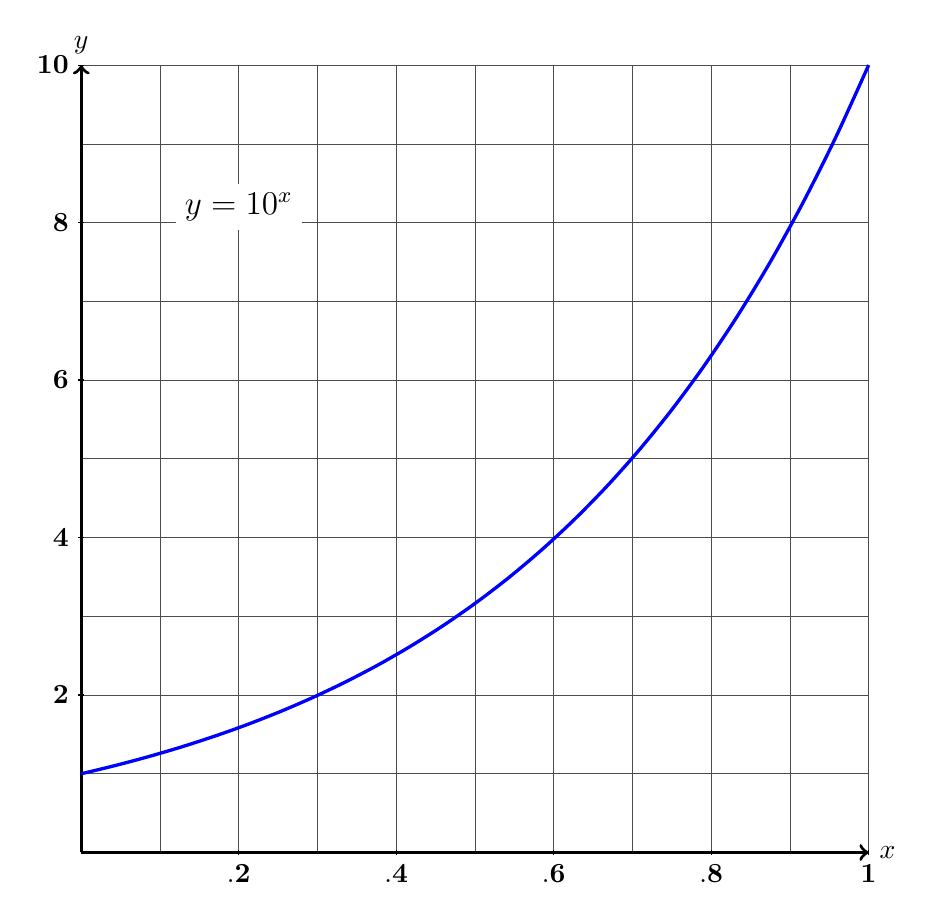
\begin{tikzpicture}
 %grid
  \draw[step=1cm,black!70,very thin] (0,0) grid (10,10);
  %axes
  \draw[very thick,->] (0,0) -- (10,0) node[anchor= west] {\bf{$x$}};
  \draw[very thick,->] (0,0) -- (0,10) node[anchor=south] {\bf{$y$}};
  \foreach \x in {.2,.4,.6,.8,1}
    \draw (10*\x cm,1pt) -- (10*\x cm,-1pt) node[anchor=north] {$\mathbf{\x}$};
  \foreach \y in {2,4,6,8,10}
    \draw (1pt,\y cm) -- (-1pt,\y cm) node[anchor=east] {$\mathbf{\y}$};
   %Function Name
   \node[black,fill=white] at (2,8.2)
   {{\large $y=10^x$}};
   %function
   \draw[scale=1.0,domain=0:10,smooth,variable=\x,blue,very thick] plot (\x,{10^(.1*\x)})
   %Code from previous exam below:
   %\draw[thick,black] plot[domain=0:10] (\x,{10^(.1*\x)})
   ;
 \end{tikzpicture}
\begin{enumerate} 
\item $\log(10) + \log(0.316)$
\vspace{40pt} \\ \phantom{.} \hfill$ \ $ \ansbox{200}{70} 
\item If $\log(y)=6.3$, then
\vspace{40pt} \\ \phantom{.} \hfill$y= \ $ \ansbox{200}{70} 
\item Find the average rate of change of $10^x$ between $x=0.7$ and $x=0.9$. 
\vspace{40pt} \\ \phantom{.} \hfill$\frac{\Delta y}{\Delta x}= \ $ \ansbox{200}{70} 
\end{enumerate} 



%%%%%%%%%%% (2)
\item ({\it 6pts}) Compute the following derivatives.
\begin{enumerate} 
\item $\displaystyle\frac{d}{dx}\left( 3x^5 - 2x^2 - 14\sqrt{x} \right)=$ \ansbox{200}{70} \vspace{120pt} \\
\item $\displaystyle\frac{d}{dx}\left( 4x^2 + 5e^{2x} - 5e^{3x} \right)=$ \ansbox{200}{70} \vspace{120pt} \\
\item $a$ and $b$ are constants. If $$f(x) = \frac{a}{\sqrt[3]{x}} - \frac{b}{(e^{x})^2}$$ 
\vspace{120pt} \\ \phantom{.} \hfill then $ \ f'(1)= \ $ \ansbox{300}{70} 
\end{enumerate}


%%%%%%%%%%% (3)
\newpage
\item ({\it 8pts}) This question is about the graph of the function
$$f(x)=2x^3 +3x^2 - 12x + 172.$$
\begin{enumerate} 
\item What is the slope of the graph at $x=0$?
\vspace{30pt} \\ \phantom{.} \hfill slope$ \ = \ $ \ansbox{200}{70} 
\item What is the equation of the tangent line to the graph at $x=2$? Please use one of the following forms: \\ $y=mx+b$ or $y=m(x-x_1)+y_1$. 
\vspace{80pt} \\ \phantom{.} \hfill$ \ y= \ $ \ansbox{200}{70} 
\item For what $x$ value (or $x$ values) does the graph have 0 slope? 
\vspace{80pt} \\ \phantom{.} \hfill$ \ x= \ $ \ansbox{200}{70} 
\item For which $x$ values is the graph $y=f(x)$ concave down? %Please circle the correct less-than or greater-than symbol below and then write the corresponding number in the box next to it. (For an answer like, ``$x<-3$,'' circle the $<$ symbol and write -3 in the box.) 
\vspace{110pt} \\ \phantom{.} \hfill \ansbox{200}{70} 
\end{enumerate}

\newpage
%%%%%%%%%%% (4)
\item ({\it 10pts}) A large Nerf ball is launched upward from the top of a cliff. Its height in meters after $t$ seconds is modeled by the equation $$h(t)=-5t^2 + 30t + 50.$$
\begin{enumerate} 
\item What is the (vertical) velocity of the ball after $t$ seconds?
\vspace{55pt} \\ \phantom{.} \hfill $ \ \ $ \ansbox{200}{70} \phantom{in}m/s 
\item What is the initial height of the ball? 
\vspace{30pt} \\ \phantom{.} \hfill $h \ = \ $ \ansbox{200}{70} \phantom{in} m
\item What is the (upward) acceleration of the ball after 5 seconds?
\vspace{50pt} \\ \phantom{.} \hfill acceleration$ \ = \ $ \ansbox{200}{70} \phantom{in}m/s$^2$
\item When is the (upward) speed of the ball 0? 
\vspace{55pt} \\ \phantom{.} \hfill at$ \ t \ = \ $ \ansbox{200}{70} \phantom{in}s
\item What was the ball's maximum height?
\vspace{30pt} \\ \phantom{.} \hfill $ \ h \ = \ $ \ansbox{200}{70} \phantom{in}m
\end{enumerate}



%%%%%%%%%%% (5)
\newpage
\item ({\it 4pts}) A bacteria colony on a petri dish is growing in a circle. After $t$ days, the radius of the circle is $t^2+2t$ mm. 
\begin{enumerate}
\item What is the area of the circle after $t$ days? \vspace{10pt}\\
\phantom{.} \hfill $A(t)=$\ \ansbox{200}{50} \phantom{i} mm$^2$\phantom{/day}
\item How quickly is the area of the circle growing after $t$ days? \vspace{10pt}\\
\phantom{.} \hfill $A'(t)=$\ \ansbox{200}{50} \phantom{i} mm$^2$/day\\
\end{enumerate}
	
	
    
    

%%%%%%%%%%% (6)    
\item ({\it 6pts}) You have 600m of fencing for a rectangular field, but the field needs to also be subdivided into 3 equal areas by fencing in addition to the perimeter. If $\ell$ and $w$ are the dimensions (length and width) of your pen, the total fencing equation below relates the length and width
    $$4\ell + 2w = 600.$$
    Here there are two extra ``lengths'' to serve as dividers between the three subdivisions. \\ 
    \begin{enumerate}
    \item You know the area of the pen in terms of $\ell$ and $w$. Express the area of the pen in terms of \underline{$\ell$ only}. \vspace{.8in}\\
    \phantom{.}\hfill$A(\ell) =$\ \ansbox{190}{50} \phantom{i} m$^2$
    \item Find the length that results in the largest area $A(\ell)$ for your field. \vspace{.9in}\\
    \phantom{.}\hfill$\ell =$\ \ansbox{190}{50} \phantom{i} m\phantom{$^2$}
    \item Use your answer in part (b) to find the maximum area for your field. \vspace{.8in}\\
    \phantom{.}\hfill $A_{\text{max}} =$\ \ansbox{190}{50} \phantom{i} m$^2$
    \end{enumerate} 
    
    \newpage
    \phantom{.}













\end{enumerate}



\end{document}

\documentclass[12pt]{article}

\usepackage{fullpage}
\usepackage{graphics}
\usepackage{tikz}
\usepackage[parfill]{parskip}
\usepackage[utf8]{inputenc}
\usepackage{etoolbox}

\newbool{alt}
\booltrue{alt}
%\boolfalse{alt}
 
% Standard things to include for math   
\usepackage{amsmath,amssymb,amsfonts,amsthm}

\usepackage{wasysym}

\usepackage{enumitem}



\usepackage{geometry}
 \geometry{
 a4paper,
 top=2cm,
 bottom=2cm,
 left=2cm,
 right=2cm,
 }




% Some of Ebrahim's definitions
\newcommand{\done}{\\\hspace*{0pt}\hfill$\blacksquare$}
\def\N{\mathbb{N}}
\def\R{\mathbb{R}}
\def\Q{\mathbb{Q}}
\def\Z{\mathbb{Z}}
\def\e{\epsilon}
\newcommand{\seq}[1]{\left(#1\right)_{n\in\N}}
\newcommand{\Euc}[1]{\mathbb{R}^{#1}}
\newcommand{\pathvarNaked}{p}
\newcommand{\pathvar}{\vec{\pathvarNaked}}
\newcommand{\pathvarAlt}{\vec{q}}
\newcommand{\exercisesList}[2]{\textcolor{ForestGreen}{Exercises from WeBWorK HW#1: #2.}}
\newcommand{\exerciseText}[1]{\textcolor{ForestGreen}{Exercise: #1}}
\def\vx{\vec{x}}
\def\vu{\vec{u}}
\def\vv{\vec{v}}
\def\vw{\vec{w}}
\newcommand{\der}[2]{\frac{\textrm{d}#1}{\textrm{d}#2}}
\newcommand{\derOp}[1]{\der{\phantom{#1}}{#1}}
\newcommand{\pder}[2]{\frac{\partial #1}{\partial #2}}
\newcommand{\pderOp}[1]{\pder{\phantom{#1}}{#1}}
\newcommand{\colvectwo}[2]{\left[\begin{array}{c}#1\\#2\end{array}\right]}
\newcommand{\colvectwoXYVEC}[2]{\left[#1\right]\,\cbv{x} + \left[#2\right]\,\cbv{y}}
\newcommand{\colvecthree}[3]{\left[\begin{array}{c}#1\\#2\\#3\end{array}\right]}
\newcommand{\colvecfour}[4]{\left[\begin{array}{c}#1\\#2\\#3\\#4\end{array}\right]}
\newcommand{\colvecfourL}[4]{\left[\begin{array}{l}#1\\#2\\#3\\#4\end{array}\right]}
\newcommand{\norm}[1]{\left|\hspace{-1.5pt}\left|#1\right|\hspace{-1.5pt}\right|}
\def\grad{\vec{\nabla}}
\newcommand{\Dir}[3]{\operatorname{Dir}(#1,#2,#3)}
\newcommand{\D}[1]{\textrm{D}#1}
\def\vn{\vec{n}}
\newcommand{\cbv}[1]{\partial_{#1}}
\newcommand{\arrayBrackets}[2]{\left[ \begin{array}{#1} #2 \end{array} \right] }

\makeatletter
\newcommand*\dotp{\mathpalette\bigcdot@{.5}}
\newcommand*\bigcdot@[2]{\mathbin{\vcenter{\hbox{\scalebox{#2}{$\m@th#1\bullet$}}}}}
\makeatother



\newcommand{\ansbox}[2]{\raisebox{-.5\height}{\framebox(#1,#2){}}}

\def\endans{\hspace{1em}\ansbox{40}{40}}


\newcommand{\NEcheckbox}{ % Put check box on northeast corner of page
\begin{tikzpicture}[remember picture,overlay] 
\path (current page.north east) ++(-1,-1) node[below left] {
{\small graded?} {\Large\Square}
};
\end{tikzpicture}
}

\newcommand{\LEFTcheckbox}{ % Put check box in the left margin
\\\begin{tikzpicture}[remember picture,overlay] 
\path ++(-2,0) node[below left] {
 {\Large\Square}
};
\end{tikzpicture}
}

\newcommand{\LEFTcheckboxOwnLine}{ % Put check box in the left margin, use this one if on own line
\begin{tikzpicture}[remember picture,overlay] 
\path ++(-2,0) node[below left] {
 {\Large\Square}
};
\end{tikzpicture}
}






\pagenumbering{gobble}
\begin{document}




% --- Score table ---

%\def\gap{\hspace*{2.5em}}
%
%\begin{tikzpicture}[overlay, remember picture]
%\path (current page.north east) ++(-1,-1) node[below left] {
%\begin{tabular}{c|c|c|c|c|c|c|c}
% 1 &  2 & 3 & 4 & 5 & 6 & 7 & $\Sigma$\\ \hline
% \gap & \gap & \gap & \gap & \gap & \gap & \gap & \gap \\
% \gap & \gap & \gap & \gap & \gap & \gap & \gap & \gap
%\end{tabular}
%};
%\end{tikzpicture}

% ---


\def\namepos{(current page.north west) ++(5,-0.8)}
\begin{tikzpicture}[overlay, remember picture]
\draw [black] \namepos rectangle ++(10,-1);
\draw [black] \namepos ++(0,-1.2) rectangle ++(10,-1);
%\draw [black] \namepos ++(0,-1.2) ++(0,-1.2) rectangle ++(10,-1);
%\draw [black] \namepos ++(0,-1.2) ++(0,-1.2) ++(0,-1.2) rectangle ++(10,-1);
\path \namepos ++(0,-0.4) node [left] {\textbf{Name:}};
\path \namepos ++(0,-0.4) ++ (0,-1.2) node [left] {\textbf{Perm:}};
%\path \namepos ++(0,-0.4) ++ (0,-1.2) ++ (0,-1.2) node [left] {\textbf{Seat Number:}};
%\path \namepos ++(0,-0.4) ++ (0,-1.2) ++ (0,-1.2) ++ (0,-1.2) node [left] {\textbf{ID Checker Name:}};
\end{tikzpicture}

\def\versionRowText{
\textit{version \ifbool{alt}{1}{2},row}
\raisebox{-3pt}{\framebox(15,15){A}}
}
\begin{tikzpicture}[overlay, remember picture]
\path (current page.north east) ++ (-2,-1.5) node [left] %{\versionRowText};
\end{tikzpicture}



\vspace{5em}

\begin{center}\textbf{Math 34A Midterm 2, Winter 2020}\end{center}
\begin{enumerate}

%%%%%%%%%%% (1)
\newpage
\item ({\it 6 pts}) Use the graph below to approximate the next three values. \\
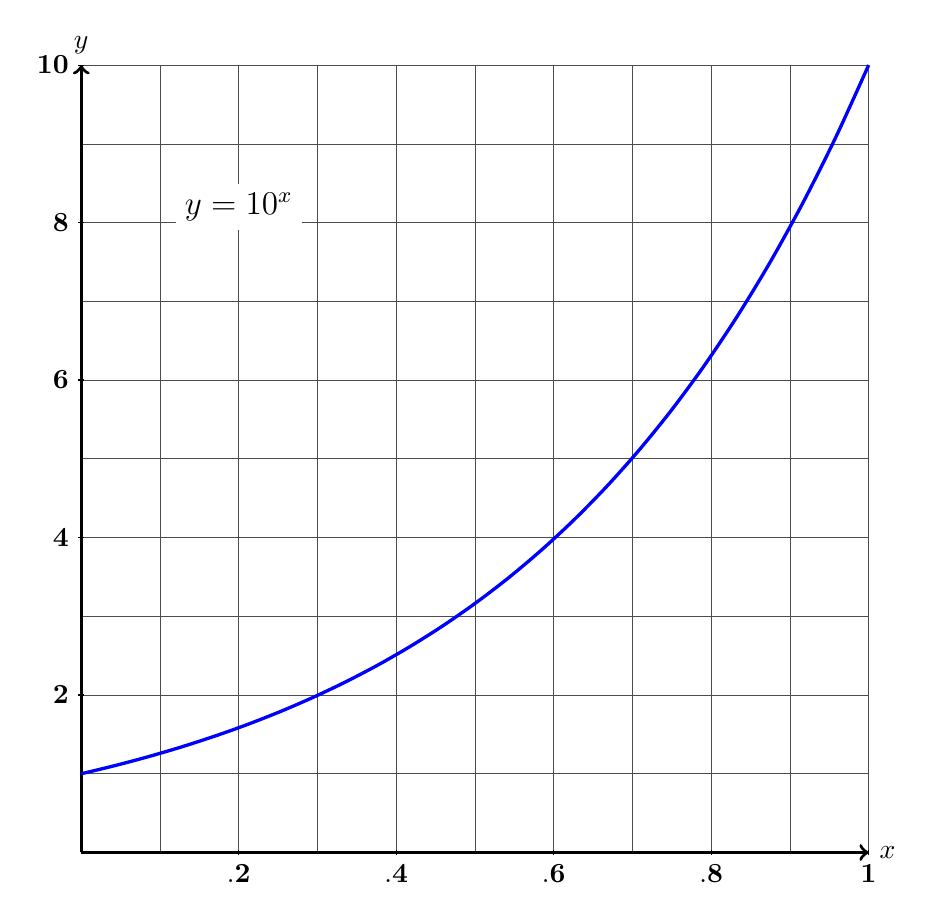
\begin{tikzpicture}
 %grid
  \draw[step=1cm,black!70,very thin] (0,0) grid (10,10);
  %axes
  \draw[very thick,->] (0,0) -- (10,0) node[anchor= west] {\bf{$x$}};
  \draw[very thick,->] (0,0) -- (0,10) node[anchor=south] {\bf{$y$}};
  \foreach \x in {.2,.4,.6,.8,1}
    \draw (10*\x cm,1pt) -- (10*\x cm,-1pt) node[anchor=north] {$\mathbf{\x}$};
  \foreach \y in {2,4,6,8,10}
    \draw (1pt,\y cm) -- (-1pt,\y cm) node[anchor=east] {$\mathbf{\y}$};
   %Function Name
   \node[black,fill=white] at (2,8.2)
   {{\large $y=10^x$}};
   %function
   \draw[scale=1.0,domain=0:10,smooth,variable=\x,blue,very thick] plot (\x,{10^(.1*\x)})
   %Code from previous exam below:
   %\draw[thick,black] plot[domain=0:10] (\x,{10^(.1*\x)})
   ;
 \end{tikzpicture}
\begin{enumerate} 
\item $\log(2/3.25)$
\vspace{40pt} \\ \phantom{.} \hfill$ \ $ \ansbox{200}{70} 
\item $10^{2.773}$
\vspace{40pt} \\ \phantom{.} \hfill$ \ $ \ansbox{200}{70} 
\item $\log(\sqrt[3]{4000})$
\vspace{40pt} \\ \phantom{.} \hfill$ \ $ \ansbox{200}{70} 
\end{enumerate} 



%%%%%%%%%%% (2)
\item ({\it 3pts}) Solve the following equations. Leave logs in your answer. 
$$7^{3x-4} = 5^{30} $$
\vspace{30pt} \\ \phantom{.} \hfill$ \ x= \ $ \ansbox{200}{70} 

%%%%%%%%%%% (3)
%\newpage
\item ({\it 6pts}) Line A goes through the points $(2,6)$, $(4,4)$. Line B has slope $\frac{2}{3}$ and goes through the point $(6,7)$. 
\begin{enumerate} 
\item What is the equation of line $A$? Give the answer in the form $y=mx + b$. 
\vspace{80pt} \\ \phantom{.} \hfill$ \ y= \ $ \ansbox{200}{70} 
\item What is the equation of line $B$? Give the answer in the form $y=mx + b$. 
\vspace{80pt} \\ \phantom{.} \hfill$ \ y= \ $ \ansbox{200}{70} 
\item What are the coordinates of the point where the lines $y=3+x$ and $y=9-x$ intersect? 
\vspace{80pt} \\ \phantom{.} \hfill$ \ (x,y)= \ $ \ansbox{200}{70} 
\end{enumerate}


%%%%%%%%%%% (4)
\item ({\it 6pts}) A square garden consists of a semicircular pond and the rest is a lawn. The length of each side is $\ell$. \\
{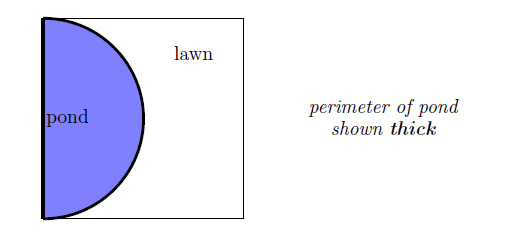
\includegraphics[width=7in]{Midterm_2_Pond_Screenshot.png} }
\begin{enumerate} 
\item Find the area of the pond in terms of $\ell$.
\vspace{55pt} \\ \phantom{.} \hfill pond area$ \ = \ $ \ansbox{200}{70} \phantom{in}
\item Find the perimeter of the pond in terms of $\ell$.
\vspace{55pt} \\ \phantom{.} \hfill perimeter$ \ = \ $ \ansbox{200}{70} \phantom{in}
\item If the area of the square is 1,600 $m^2$, then find the area of the lawn. (The answer does not depend on $\ell$.) 
\vspace{50pt} \\ \phantom{.} \hfill lawn area$ \ = \ $ \ansbox{200}{70}$\ m^2$ 
\end{enumerate}



%%%%%%%%%%% (5)
\newpage
\item ({\it 6pts}) Initially can A contains 6 liters of red paint and can B contains 12 liters of blue paint. I pour 1/2 of the red paint into can B. 
\begin{enumerate} 
\item What is the percentage of blue paint in can B?
\vspace{120pt} \\ \phantom{.} \hfill \ansbox{200}{70} \%
\item After mixing the paint in can B, I pour 1/2 of the paint in can B into can A. How many liters of paint are now in can A? 
\vspace{120pt} \\ \phantom{.} \hfill \ansbox{200}{70} L
\item How many liters of blue paint are now in can A? 
\vspace{120pt} \\ \phantom{.} \hfill \ansbox{200}{70} L
\end{enumerate}
 
%%%%%%%%%%% (6)
\newpage

\item ({\it 3 points}) Write out the following sum. 
$$\sum_{n=3}^7 (n-1)(n+1)$$
= \ \ansbox{450}{70}

%%%%%%%%%%% (7)
%\newpage
\item ({\it 4 points}) What are the following limits? 
\begin{enumerate} 
\item {\large $\underset{h \rightarrow 0}{\lim} \ \ $} {\Large $\frac{7+4h-7}{h}$} \\ \\ \phantom{.} \hfill\ansbox{140}{70} \\ \\  
\item {\large $\underset{h \rightarrow 0}{\lim}$} \ \ {\large $\frac{50 + 20h + 2h^2 - 50}{h}$} \\ \\ \phantom{.} \hfill\ansbox{140}{70} \\ \\  
\end{enumerate}


%%%%%%%%%%% (8)
\item ({\it 3 points}) 
Find the average speed of a race car over the time period from 2 seconds to 2.1 seconds if $f(t) =t^2$ is the distance in meters from the starting line $t$ seconds after the start. 
\vspace{210pt}\\
\phantom{.} \hfill\ansbox{120}{70} \ $m/s$ 


%%%%%%%%%%% (9)
%\item ({\it 3 points})















\end{enumerate}



\end{document}

